\documentclass[12pt, a4paper, UTF8, fontset=windows]{ctexbook}
\usepackage{amsmath, amsthm, amssymb, amsfonts, bm, color, fancyhdr, framed, geometry, graphicx, hyperref, lastpage, listings, mathrsfs, xcolor}


\linespread{1.5}
\definecolor{shadecolor}{RGB}{241, 241, 255}
\newcounter{problemname}
\newenvironment{problem}{\begin{shaded}\stepcounter{problemname}\par\noindent\textbf{Q\arabic{problemname}.}}{\end{shaded}\par}
\newenvironment{solution}{\par\noindent\textbf{Ans.}}{\par}

\geometry{left=20mm,right=20mm, top=20mm, bottom=22mm} % 页边距
\setlength{\headheight}{15pt}
\pagestyle{fancy} % 设置页脚页眉
\rhead{Assignment2} % 页眉右边
% \noindent % 取消首段缩进

\definecolor{mygreen}{rgb}{0,0.6,0}
\definecolor{mygray}{rgb}{0.5,0.5,0.5}
\definecolor{mymauve}{rgb}{0.58,0,0.82}
% 代码设置
\lstset{ 
backgroundcolor=\color{white},      % choose the background color
basicstyle=\footnotesize\ttfamily,  % size of fonts used for the code
columns=fullflexible,
tabsize=4,
breaklines=true,               % automatic line breaking only at whitespace
captionpos=b,                  % sets the caption-position to bottom
commentstyle=\color{mygreen},  % comment style
keywordstyle=\color{blue},     % keyword style
stringstyle=\color{mymauve}\ttfamily,  % string literal style
frame=single,
rulesepcolor=\color{red!20!green!20!blue!20},
language=sql,
xleftmargin=3em,
xrightmargin=3em
}


\begin{document}

\cfoot{\thepage\ / \pageref{LastPage}} % 页眉中间位添加内容:页码/总页码

\thispagestyle{empty}

\begin{figure}[t]
    \centering
    
\includegraphics[width=6cm]{../../src/images/logo.jpg}
\end{figure}

\vspace*{\fill}
    \begin{center}
        \Huge\textbf{Assignment2}
    \end{center}
\vspace*{\fill}

\begin{table}[b]
    \centering
    \large
    \begin{tabular}{ll}
    \textbf{课程:} & 数据库原理与应用 \\
    \textbf{姓名:} & 雷翔 \\
    \textbf{学号:} & 2053932 \\
    \textbf{时间:} & 2023年4月 \\
    \end{tabular}
\end{table}


\newpage

\setcounter{page}{1} % 页码从当前页开始

\begin{problem}
    4.15 请重写查询

    \begin{lstlisting}
    select *
    from section natural join classroom;
    \end{lstlisting}
\end{problem}

\begin{solution}
    \begin{lstlisting}
    select *
    from section join classroom using (building, room_number);
    \end{lstlisting}    
\end{solution}


\begin{problem}
    5.15 请考虑具有两个关系的雇员数据库
    
    $employee \left( employee_name, street, city \right)$

    $works \left( employee_name, company_name, salary \right)$

    其中主码用下划线标出。请编写一个 avg\_salary 函数,它以公司名称作为参数,并查找该公司员工的平均工资。\ 
    然后,请使用该函数编写一条 SQL 语句,来查询员工平均工资高于 "First Bank" 平均工资的公司。 
\end{problem}

\begin{solution}
    \begin{lstlisting}
    -- 定义函数
    create function avg_salary(company_name varchar(20)) 
    returns int
    begin
        declare avg_salary_num int;
        select avg(salary) into avg_salary_num
        from works
        where works.company_name = avg_salary.company_name;
        return avg_salary_num;
    end

    -- 调用函数
    select distinct company_name, avg_salary(company_name)
    from works
    where avg_salary(company_name) > avg_salary('First Bank');
    \end{lstlisting}

    
    \newpage
    以下代码在 MySQL 环境测试成功
    \begin{lstlisting}
    -- 定义函数
    CREATE DEFINER=`root`@`localhost` FUNCTION `avg_salary`(company_name VARCHAR(20)) RETURNS int
    BEGIN
        DECLARE avg_salary_num INT;
        SELECT avg(salary) INTO avg_salary_num
        FROM works
        WHERE works.company_name = company_name;  
        -- MySQL 中引用参数不需要函数名.xxx
        RETURN avg_salary_num;
    END

    -- 调用函数
    SELECT DISTINCT company_name, avg_salary(company_name)
    FROM works
    WHERE avg_salary(company_name) > avg_salary('First Bank');
    \end{lstlisting}
\end{solution}

\newpage

\begin{problem}
   6.23 为全球包裹递送公司(例如 DHL 或者 FedEX)设计一个数据库。致据库必须能够追踪寄件客户和收件客户,有些客户可能两者都是。\ 
   每个包裹必须是可标识且可追踪的,因此数据库必须能够存储包裹的位置以及它的历史位置。位置包括卡车、飞机、机场和仓库。

   你的设计应该包括 E-R 图、关系模式的集合,以及包括主码和外码约束在内的一系列约束。
\end{problem}


\begin{solution}
    E-R 图
    \begin{figure}[htbp]
        \centering
        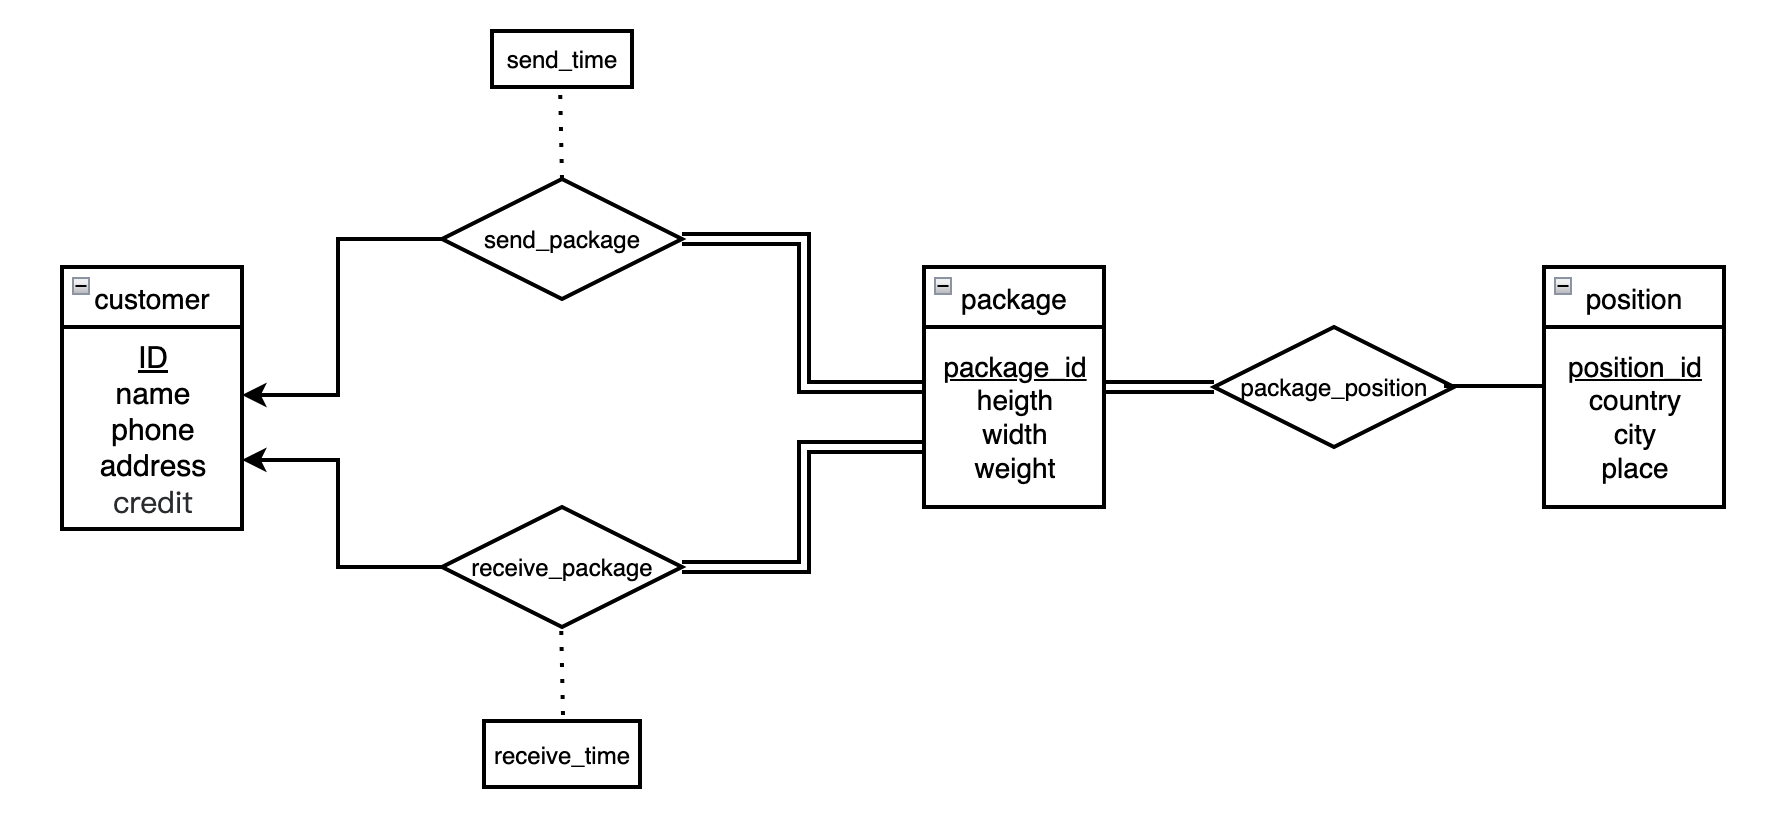
\includegraphics[width=0.8\textwidth]{../../src/images/hw2-option1.png}
        \caption{方法一}
    \end{figure}

    \begin{figure}[htbp]
        \centering
        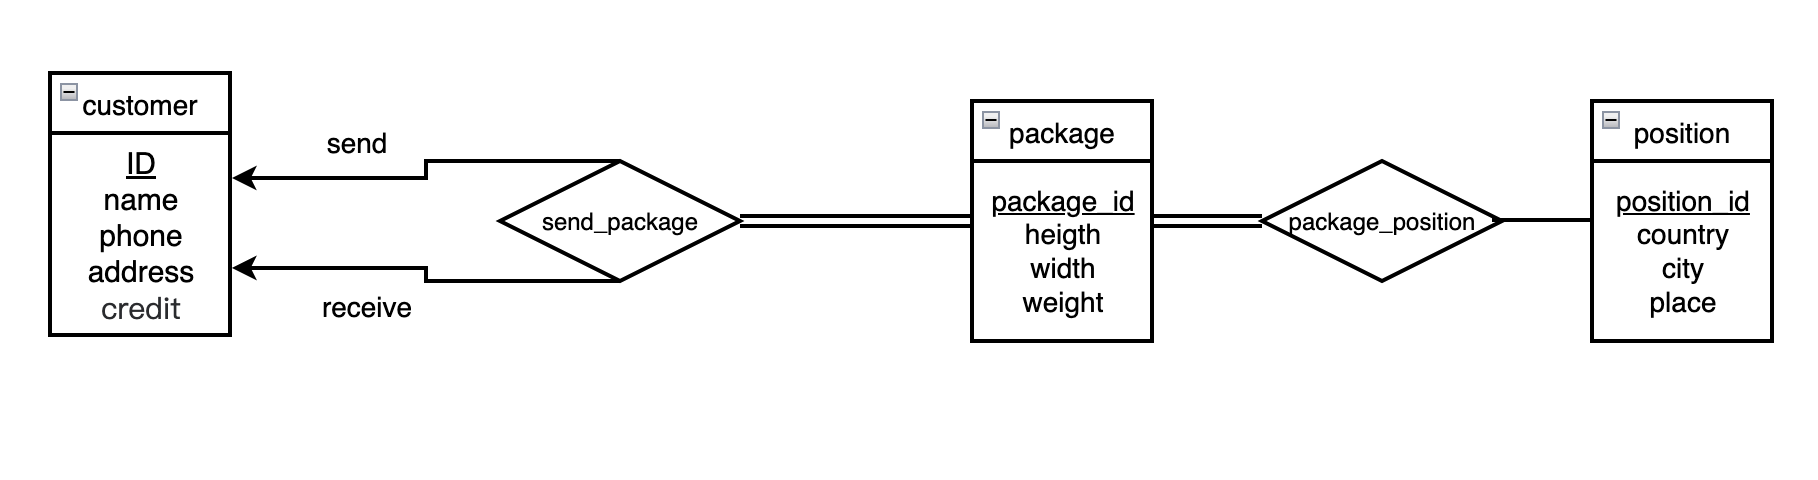
\includegraphics[width=0.8\textwidth]{../../src/images/hw2-option2.png}
        \caption{方法二}
    \end{figure}

    关系模式

    \begin{lstlisting}
    -- 三个实体集
    customer(
        customer_id,
        customer_name,
        customer_phone,
        customer_address,
        customer_credit,
        primary key(customer_id)
    )
    package(
        package_id,
        height,
        width,
        weight,
        primary key(package_id)
    )
    position(
        position_id,
        country,
        city,
        place,
        primary key (position_id, package_id),
    )
    -- 两个联系集
    send(
        send_customer_id,
        receive_customer_id,
        package_id,
        send_time,
        receive_time,
        primary key (send_customer_id, receive_customer_id, package_id),
        foreign key (send_customer_id) references customer(customer_id),
        foreign key (receive_customer_id) references customer(customer_id),
        foreign key (package_id) references package(package_id)
    )
    package_position(
        package_id,
        position_id,
        primary key (package_id, position_id),
        foreign key (package_id) references package(package_id),
        foreign key (position_id) references position(position_id)
    )
    \end{lstlisting}

\end{solution}

\newpage

\begin{problem}
    7.26 请考虑下面提出的用于函数依赖的规则:若 $\alpha \to \beta$ 且 $\gamma \to \beta$,则 $\alpha \to \gamma$。 \
    通过给出一个关系 r,它满足 $\alpha \to \beta$ 和 $\gamma \to \beta$ 但并不满足 $\alpha \to \gamma$,来证明这条规则不是有效的。 
\end{problem}

\begin{solution}
    设 $\alpha$、$\beta$ 和 $\gamma$ 分别对应关系 r 中属性 A、B 和 C,则有如下关系:
    \vspace{2mm}  % 指定高度,添加空行

    \begin{tabular}{c|c|c|c}
        \hline
        r & A & B & C \\
        \hline
        & $a_1$& $b_1$&$c_1$\\
        & $a_1$& $b_1$&$c_2$\\
        \hline
    \end{tabular}

    \vspace{2mm}  % 指定高度,添加空行
    在上面的关系中,有两对元组,分别是 ($a_1, b_1, c_1$) 和 ($a_1, b_1, c_2$)。

    对于 r 中的所有元组,在 A 上值相等的元组在 B 上的值也相等,因此 $\alpha \to \beta$,\
    同理,在 C 上值相等的元组在 B 上的值也相等,因此 $\gamma \to \beta$。 \
    但在 A 上值相等的元组在 C 上的值不相等,因此 $\alpha \to \gamma$ 不成立。

    综上,这条规则不是有效的。
   
\end{solution}


\begin{problem}
    7.27 请用阿姆斯特朗公理来证明分解律的有效性。
\end{problem}

\begin{solution}
    分解律:若 $\alpha \to \beta \gamma$ 成立,则 $\alpha \to \beta$ 和 $\alpha \to \gamma$ 也成立。 
    
    $\beta \subseteq \beta \gamma \Rightarrow \beta \gamma \to \beta$ (1)
    
    $\gamma \subseteq \beta \gamma \Rightarrow \beta \gamma \to \gamma$ (2)
    
    根据 (1) 和 $\alpha \to \beta \gamma$,由传递律可得 $\alpha \to \beta$

    同理,根据 (2) 和 $\alpha \to \beta \gamma$,由传递律可得 $\alpha \to \gamma$   

    综上,分解律是有效的。
\end{solution}

\end{document}